\section{Problems}

[Convex Optimization, Mean/Medium/Mode, Preparation for Learning Loss Functions]

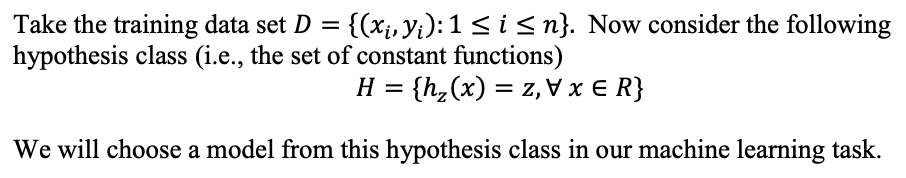
\includegraphics[width=1\textwidth]{media/problems_intro.png}

\subsection{Question One}
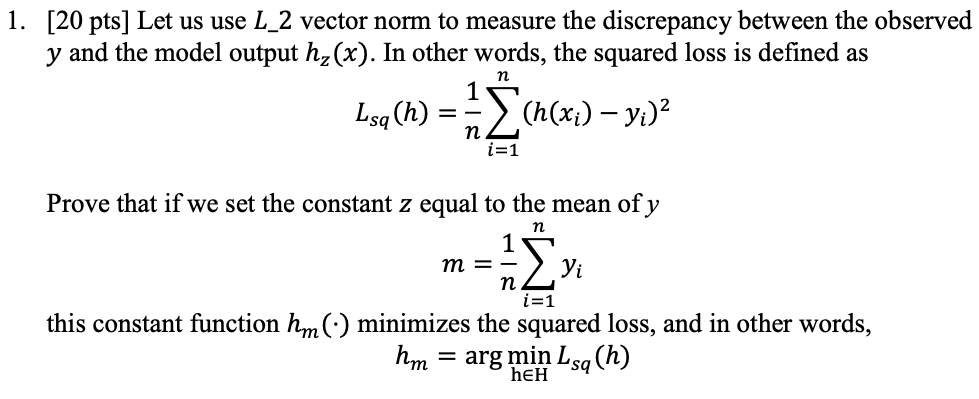
\includegraphics[width=1\textwidth]{media/q1.png}

We are given our model from the hypothesis class as:
\begin{align}
    H = \{ h_z(x) = z, \, \forall \, x \in \mathbb{R} \} \label{eq:hypothesis_class}
\end{align}

Our squared loss function is given as:
\begin{align}
    L_{sq}(h) &= \frac{1}{n} \sum_{i=1}^n (h(x_i)-y_i)^2 \label{eq:sq_loss} \nonumber \\
    &= \frac{1}{n} \sum_{i=1}^n (z-y_i)^2 && \text{(from Eq. \ref{eq:hypothesis_class})}
\end{align}

This is a convex optimization problem. From the lectures, we know that the optimality condition is given as: 
\begin{align}
    \min_{x \in \mathbb{R}^n} \Rightarrow \nabla_x f(x^*) = 0 \label{eq:optimization_condition}
\end{align}

Therefore, we first take the derivative of our loss function, Eq. \ref{eq:sq_loss}.
\begin{align}
    \frac{\partial L_{sq}(h)}{\partial z} &= \frac{\partial}{\partial z} \Big(\frac{1}{n} \sum_{i=1}^{n} (z-y_i)^2 \Big) \nonumber \label{eq:q1_deriv} \\
    &= \frac{1}{n} \frac{\partial}{\partial z} \sum_{i=1}^{n} (z-y_i)^2  \nonumber \\
    &= \frac{1}{n} \sum_{i=1}^{n} 2 \cdot(z-y_i)  \nonumber \\
    &= \frac{2}{n} \sum_{i=1}^{n} (z-y_i) 
\end{align}

We then set the derivative (Eq. \ref{eq:q1_deriv}) to 0 to optimize and solve.
\begin{align}
    0 &= \frac{2}{n} \sum_{i=1}^{n} (z-y_i) \nonumber \label{eq:q1_optimize} \\
    0 &= \sum_{i=1}^{n} (z-y_i) \nonumber \\
    0 &= \sum_{i=1}^{n} z - \sum_{i=1}^{n} y_i \nonumber \\
    0 &= n \cdot z - \sum_{i=1}^{n} y_i \nonumber && \text{($z$ is a constant)}\\
    n \cdot z &= \sum_{i=1}^{n} y_i \nonumber \\
    \Rightarrow z &= \frac{1}{n }\sum_{i=1}^{n} y_i
\end{align}

$\therefore$ We have shown in Eq. \ref{eq:q1_optimize} that $z = m$, the mean of $y$, when minimizing the squared loss function, $L_{sq}(h)$ (Eq. \ref{eq:sq_loss}).

$\therefore h_m(\cdot) = h_z(x) = z = m = \frac{1}{n }\sum_{i=1}^{n} y_i$ minimizes the squared loss function, and hence $h_m = \text{arg min}_{h \in H} L_{sq}(h)$.

\subsection{Question Two}
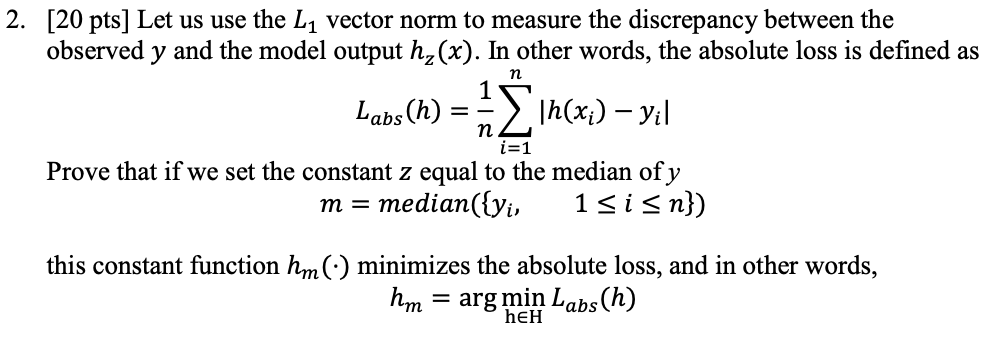
\includegraphics[width=1\textwidth]{media/q2.png}

Our absolute loss function is given as:
\begin{align}
    L_{abs}(h) &= \frac{1}{n} \sum_{i=1}^n |h(x_i)-y_i| \label{eq:abs_loss} \nonumber \\
    &= \frac{1}{n} \sum_{i=1}^n |z-y_i| && \text{(from Eq. \ref{eq:hypothesis_class})}
\end{align}

Following a similar procedure as the previous question, we treat this as a convex optimization problem, and take the derivative of Eq. \ref{eq:abs_loss} in order to find the value of $z$ that minimizes it.

\begin{align}
    \frac{\partial L_{abs}(h)}{\partial z} &= \frac{\partial}{\partial z} \Big(\frac{1}{n} \sum_{i=1}^n |z-y_i| \Big) \nonumber \label{eq:q2_deriv1} \\
    &= \frac{1}{n} \frac{\partial}{\partial z} \sum_{i=1}^n |z-y_i|
\end{align}

Let's think carefully about what's happening here. We want to find the value of $z$ that minimizes $L_{abs}(h)$ (Eq. \ref{eq:abs_loss}). Examining the derivative in Eq. \ref{eq:q2_deriv1} further:
\begin{align}
    \frac{\partial}{\partial z} |z-y_i| &= \begin{cases} 
        1 & \text{if } z > y_i \\
        0 & \text{if } z = y_i \\
        -1 & \text{if } z < y_i
    \end{cases} \nonumber \label{eq:q2_deriv2} 
\end{align}

This indicates that when $z=y_i$, the gradient is equal to 0, which means $L_{abs}(h)$ is minimized. Given that $L_{abs}(h)$ is summing the absolute differences between our $z$ and every $y_i$, $z=y_i$ only when $z$ is the median of $y$. We know that the median is the middle point of all the values in $y$ arranged in ascending order (for example if $y={1,2,4,5,7}$, then the median of $y$ will be 4). Therefore if our $z$ is set to the median value of $y$, then the derivative of each $|z-y_i|$ will be equal to 0, which minimizes $L_{abs}(h)$ according to the optimality condition (Eq. \ref{eq:optimization_condition}).

$\therefore$ We have shown if that $z = m$, the median of $y$, then the absolute loss function, $L_{abs}(h)$ (Eq. \ref{eq:abs_loss}) is minimized.

$\therefore h_m(\cdot) = h_z(x) = z = m =$ median(y) minimizes the absolute loss function, and hence $h_m = \text{arg min}_{h \in H} L_{abs}(h)$.

\subsection{Question Three}
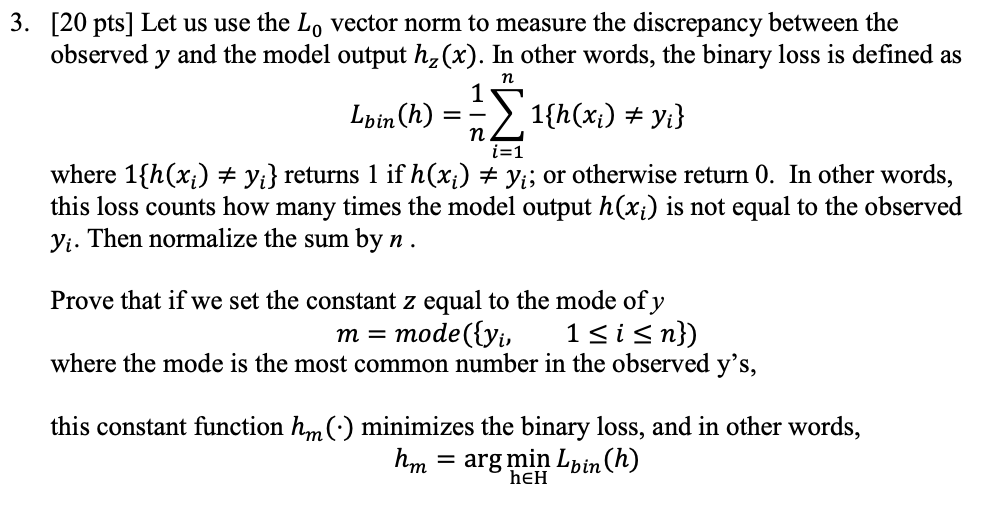
\includegraphics[width=1\textwidth]{media/q3.png}

Our binary loss function is given by:

\begin{align}
    L_{bin}(h) &= \frac{1}{n} \sum_{i=1}^n 1 ( h(x_i) \neq y_i )  \nonumber \\
    &= \frac{1}{n} \sum_{i=1}^n 1 ( z \neq y_i ) && \text{(from Eq. \ref{eq:hypothesis_class})} 
\end{align}

Once again, we want to solve for the optimality condition (Eq. \ref{eq:optimization_condition}) and therefore could take the derivative of the binary loss function. However, let's think more deeply about this. $L_{bin}(h)$ measures the normalized total number of times that $z \neq y_i$. Effectively, this is what we can re-write the binary loss function as:
\begin{align}
    L_{bin}(h) &= \frac{1}{n} \sum_{i=1}^n \begin{cases} 
        1 & \text{if } z \neq y_i \\
        0 & \text{if } z = y_i
    \end{cases} \nonumber \label{eq:q3_deriv2} 
\end{align}

The value of $L_{bin}(h)$ will be minimized when we have more occurrences of $z = y_i$ because $\sum_{i=1}^n \Rightarrow 0 + 0 + ...$ is lower than if we have more occurrences of $z \neq y_i$, in which case $\sum_{i=1}^n \Rightarrow 1 + 1 + ...$, which produces a higher value for $L_{bin}(h)$. Logically then, it makes sense that $L_{bin}(h)$ is minimized when the value of $z$ is equal to $m$ (the mode of $y$, i.e. the most-frequently occurring value in $y$). 

Therefore if our $z$ is set to the mode value of $y$, then there will be more occurrences of the value 0 in the summation part of the binary loss, which inevitably leads to the lowest (therefore most optimal) value of $L_{bin}(h)$.

$\therefore$ We have shown if that $z = m$, the mode of $y$, then the binary loss function, $L_{bin}(h)$ is minimized.

$\therefore h_m(\cdot) = h_z(x) = z = m =$ mode(y) minimizes the binary loss function, and hence $h_m = \text{arg min}_{h \in H} L_{bin}(h)$.